\chapter{Results}
\label{chapter:Chapter 5}
\lhead{Chapter 5. \emph{Results}}

\section{Experiment 1 - Overall Description.}
The experiment conducted on this Chapter, were conducted by injecting data from the Data-Set described in XX, in the Developed Framework.

The validation of the results presented in this Chapter, can only truly occur with the proper validation of a Maritime Officer, as the reported Anomalies presented in this work must not be interpreted as an actual real Maritime illegality, but only as a possible Anomaly. 

In this Section we present the results leading from experiences conducted in order to validate the operational capabilities of the Framework.

\section{Hardware Used}
\todo[inline]{this will not be a section, will be presented in Chapter intro.}

\section{Data Validation Experiment}
\label{section: Experiment Data Val}
The Data Validation Experiment we accessed the performance Data-Ingestion capability of the developed Framework. In order to achieve this, we provided a real NMEA feed as input to our the Data Ingestion Module from the developed \emph{MAD-F}.

We allowed the Framework to be executed for five straight days, thus ingesting pre-processing and wrangling the provided AIS NMEA into Behavioural Points. We then stored the $BPs$ in the Trajectory Extraction Cassandra Data-Base.
As the messages were being received in real-time the MAD-F decoded the NMEA feed into a readable format, from which the irrelevant features for the developed Framework.
\todo[inline]{Change to the BP simulation scenario}
From the 5 days of data acquiring, we received NMEA AIS messages from a total of $5563$ different Vessels, leading to a grand total of $2,259,615$ NMEA messages.

After the messages were decoded into a set of features, as the used NMEA AIS feed did not broadcast the Vessel Type of the Vessel that generated this message. The Vessel Static Information, namely the Vessel Type and country of origin were scrapped using using the developed \emph{Vessel Type Scrapper}. From the $5563$, $6$ Vessels were not considered as their static information, namely their MMSI was either not found or their MMSI was representative of more than one Vessel. The latter, represents an abnormal situation which could be denominated Spoofing, as represented by the authors in \cite{Ray2015DeAISRisks} or in \footnote{http://globalfishingwatch.org/data/spoofing-one-identity-shared-by-multiple-vessels}. This is a occurring problem when handling AIS data. 

\begin{figure}[H]
	\centering
	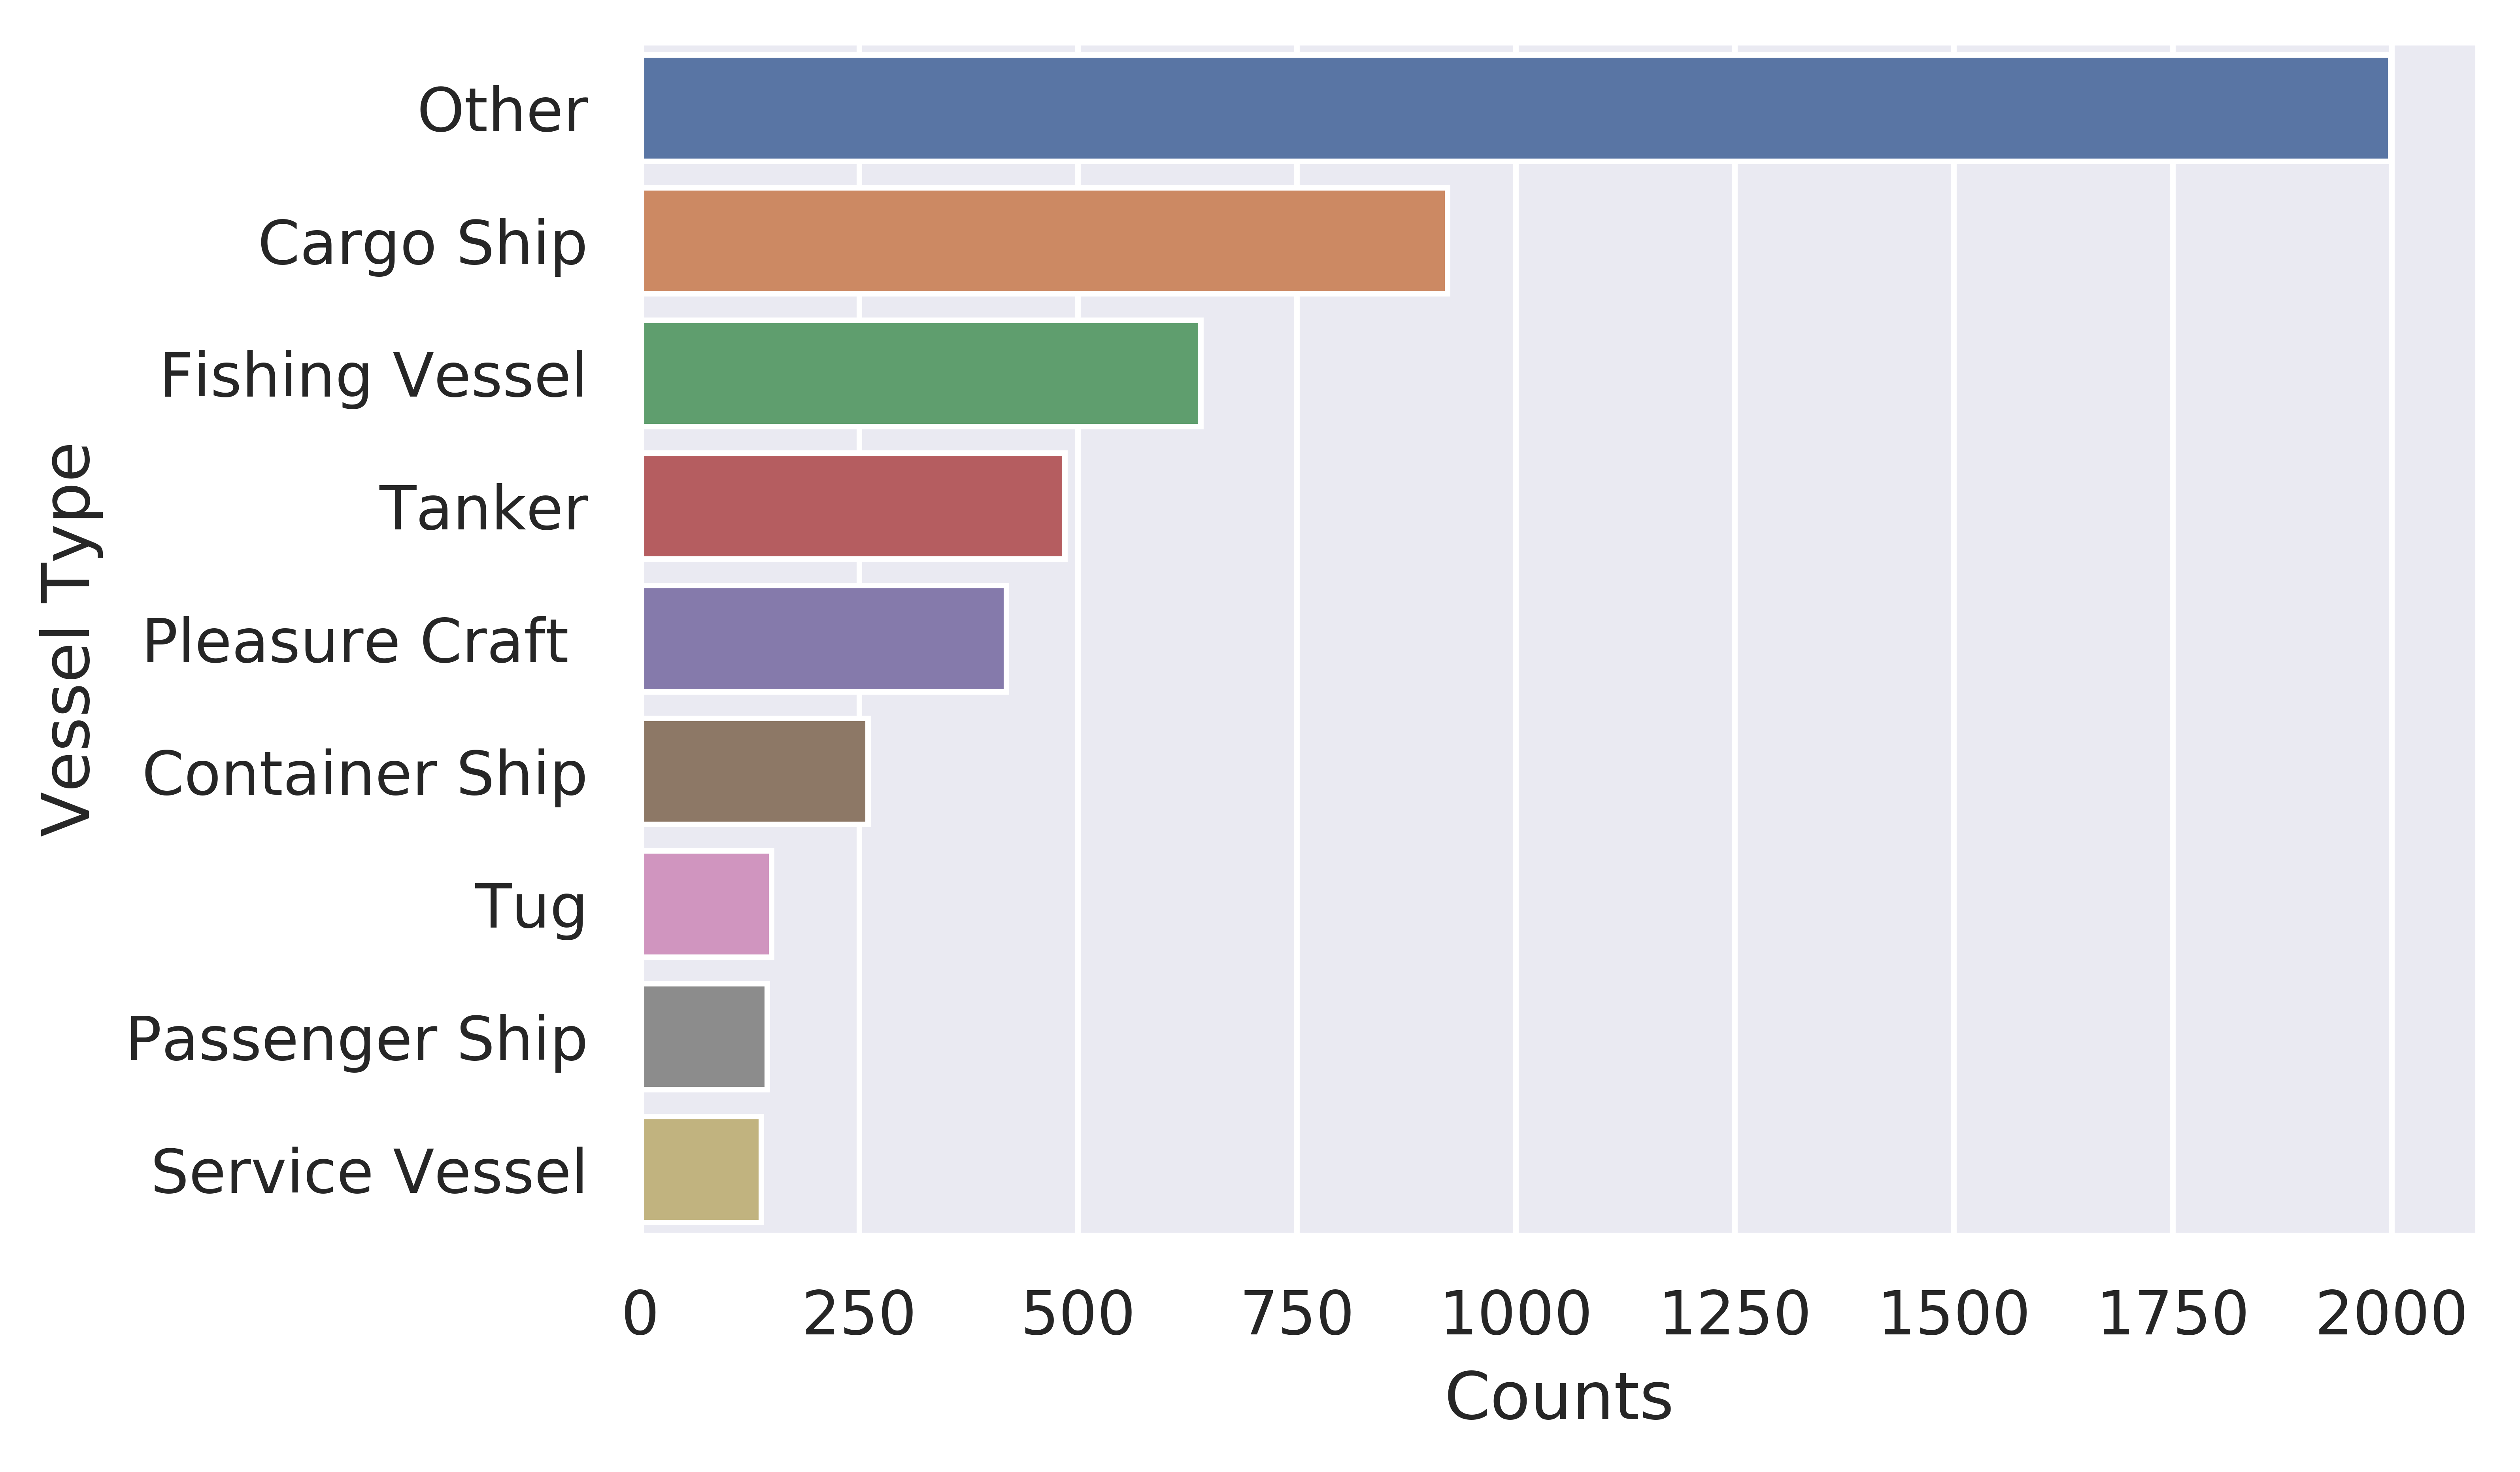
\includegraphics[scale = .7]{figures/Ch5/DataValidationVesselType.png}
    \caption{Vessel Type distribution of $5157$ Vessels.}
    \label{fig: 5 Vessel Type Distribution}
\end{figure}

\todo[inline]{talk about ports}

Another feature calculated on this module was the point-based closest distance to coast and ports. This calculation for this Experiment was done for every received NMEA AIS message. In Table XX we present a post validation of the closest Ports for every received message. This was done as a way to validate if whether the closest Ports seems plausible, as a validation message to message would be impractical. Thus, in Table XX we present the subset of top most frequent closest ports from the $69$ total possible Ports, which are plotted in Orange in figure XX.

\begin{table}[H]
\centering
\caption{Most Frequent Closest Ports Counts.}
\label{Table: 5 Closest Ports}
\begin{tabular}{@{}lcc@{}}
\toprule
Port Name & Counts & Counts(\%) \\ \midrule
Lisboa & 142,464 & 6,3\% \\
Villa Garcia De Arosa & 112,254 & 5\% \\
Europa Point(Gibraltar) & 109,273 & 4,8\% \\
Lagos & 107358 & 4,7\% \\
Las Palmas & 106,116 & 3,5\% \\
Cadiz & 79,577 & 3,5\% \\
La Corunha & 78,929 & 3,5\% \\
Malaga & 65,227 & 2,9\% \\
Vigo & 64,759 & 2,9\% \\
Faro & 62,925 & 2,9\% \\ \bottomrule
\end{tabular}
\end{table}

\begin{table}[H]
\centering
\caption{Most Frequent Closest Countries Counts.}
\label{Table: 5 Closest Countries}
\begin{tabular}{@{}lcc@{}}
\toprule
Country & Counts & Counts(\%) \\ \midrule
Spain & 1,306,436 & 58\% \\
Portugal & 663,841 & 29\% \\
Morocco & 259,776 & 11\% \\
Gibraltar & 26,885 & 1\% \\
France & 2,516 & 0.1\% \\
Cabo Verde & 161 & 0.007\% \\ \bottomrule
\end{tabular}
\end{table}
done to decoded set of features another the was the calculation of the  

The all ready pre-processed AIS Messages were then stored as $BPs$

The scrapped information was stored in a internal module cache, 

\begin{figure}[H]
	\centering
	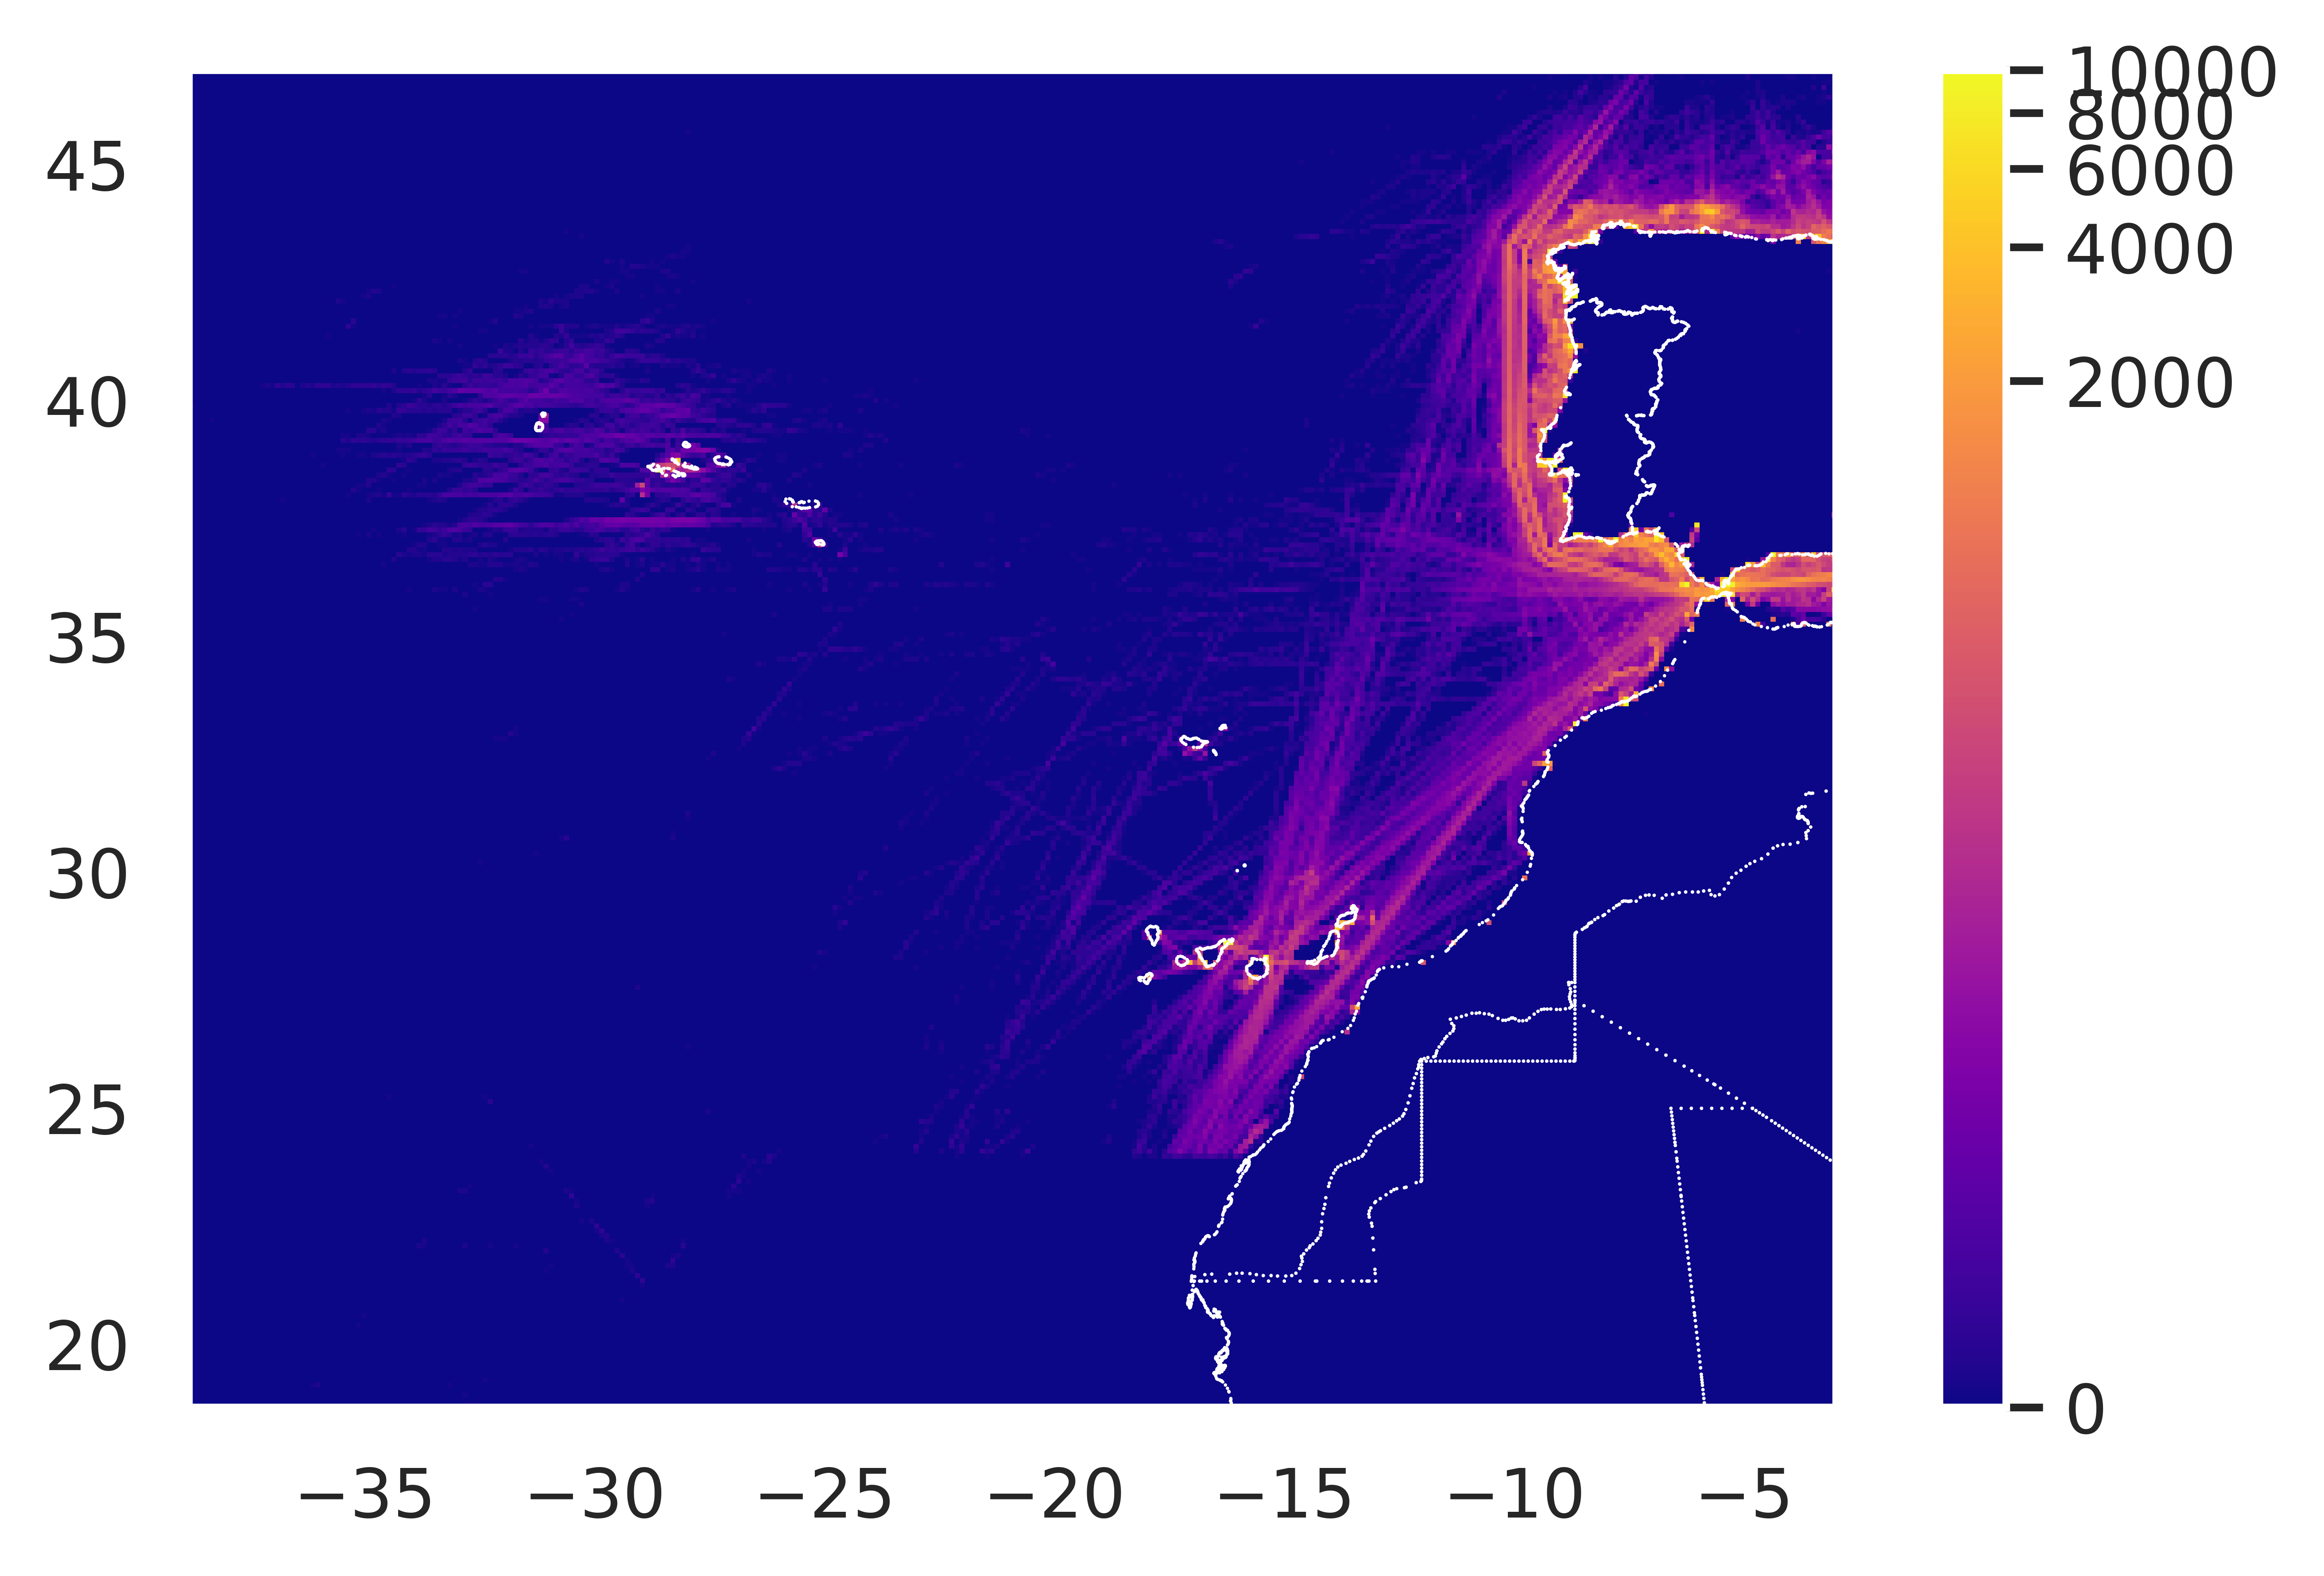
\includegraphics[scale = 1]{figures/Ch5/ThesisExpDensity.png}
    \caption{Density map, with all the aprox. $2.2$ Milion points.}
    \label{fig: 5 Exp1DensityMap}
\end{figure}

From this messages 

Validate the proper aquirement of real time data.

Simply done by leating the "System"/Framework aquiring data for 2 whole straigth days from different real time NMEA feeds from the portugal coast area.

We calculate the distance to Shore and Port

We get the Vessel Characteristics namely the vessel type, using the Scrapper for the Vessels we did not had this information provided...

PRESENT THE RESULTS FOR DISTANCE TO COAST ETC ETC...

WE SAVED THE XXX AMMOUNTS OF DATA IN THE DB FOR ANY FUTURE USE...


\section{Rule Based Anomaly Detection Experiment}
\label{section: Rule Based Anomaly Detection Experiment}

This experiment was conducted, to validate the real time capabilities of the Rule Based Anomaly Detection Module. In order to validate the capabilities of this module, we focused this experiment on the validation by analysis of the Anomalies generated by the module, and whether the module could function in near-real time or not.

To tackle this problem, we injected the resulting $BPs$ from the Experiment \ref{section: Experiment Data Val} in the RBADS module. This was done as when using the real-time data NMEA feeds we from the PTN we loose control of the incoming data, and for the validation of this experiment 

As the results from the experiment above were stored as trajectories, in order to not be dependent of new incoming data to validate the functionalities of the RBADS, we developed a $BP$ simulator, only used in this experiment.

The simulator gathers $BPs$ from the trajectories (or a group of) stored in the trajectory extraction data-base, and send this $BPs$ to the RBADS, simulating as they were new coming $BPs$ from the Feature Extraction Module, as we present in FigXX NEED TO DO THIS....

\begin{figure}[H]
	\centering
	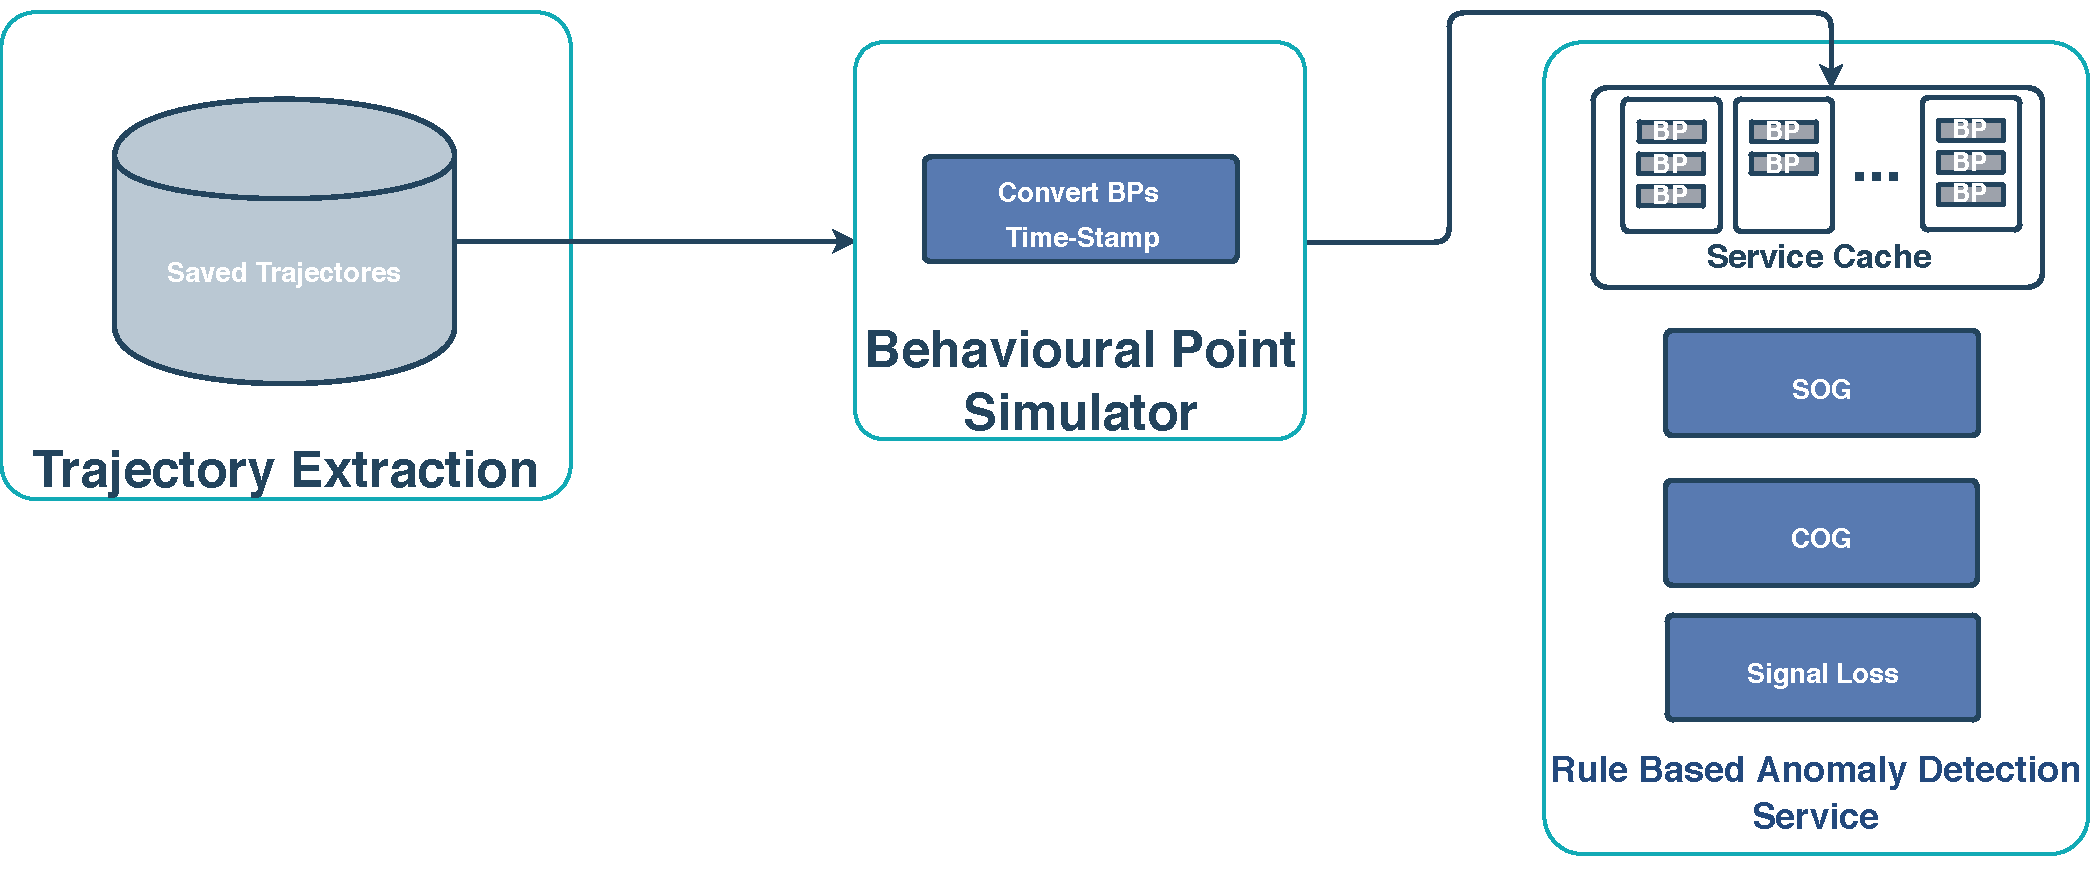
\includegraphics[scale = .3]{figures/Ch5/SRM-Exp-Simulator.pdf}
    \caption{BPs Simulator.}
    \label{fig: 5 BPs Simulator}
\end{figure}



The simulator worked by setting the a \textbf{Initial-Simulated-Time} as if it was the current Time. This 
For this Experiment the \textbf{Initial-Simulated-Time} was set first received $BP$ from the Experiment \ref{section: Experiment Data Val}, which was XXXXXXTODOXXXXXX.

Thus, we ran RBADS with the simulator setted to a speed of X, and with the RBADS parameters represented in table XX.

\missingfigure[]{Table RBADS paramenters XX}

With the parameters described above, we found XX anomalies and ALALALAL AAHAHH AJAJAJ need to do the simulation

\section{Anomaly Detection Service Experiment}
Anomaly Detection Service Experiment was for this work, the procedure we took in order to access the functionalities developed in this Module. The conduction of this experiment was similar to the Experiment \ref{section: Rule Based Anomaly Detection Experiment}, although as the motive for the development of this module was to access huge batches of data, we didn't conduct this experiment with the same Data neither the same method of Simulating the reception of Data, presented in \ref{section: Rule Based Anomaly Detection Experiment}.

This, experiment was firstly conducted with the Data-Set used for the Data-Analysis presented in XXX. This was done in order to truly access the performance of the developed Anomaly Detection Service. Thus, we ran the Anomaly Detection Service with the configurations presented under in Table XX, with a Set of 18,84 Million  $BPs$ from 4555 different Vessels. 
Whats to note in this experiment is that if this set of $BPs$ was to be stored in files as a pre-processed Data-Set they would occupy nearly 2 Gigabytes if stored as .csv type files.

The ADS presenting 2 different types of anomalies, we divided this experiment in two the Rendezvous detection and the Wrong Status Validation. Thus in the following subsections, we present the results (being the anomalies generated) and the performance of each sub experiment.


\subsection{ADS - Rendezvous Experiment}
\label{subsection: ADS - Rendezvous Experiment}
This subsection, shows the results and our analysis of the results obtained for the Rendezvous Experiment. with the whole already prepossessed Data-Set.
We conducted this Experiment on the all-ready pre-processed Data-Set(SECTION XX REF), with the Parameters represented in Table XX.

\begin{table}[H]
\centering
\caption{Anomaly Detection Service - Rendezvous input parameters.}
\label{Table: 5 ADS Rendezvous input paramenters.}
\begin{tabular}{@{}cccc@{}}
\toprule
Rendezvous Parameter & BPs & Time-Window & Distance Threshold \\ \midrule
                    & 18M & 10 min.     & 100 yards         \\ \bottomrule
\end{tabular}
\end{table}

The whole Experiment took 150 Seconds to execute with the Hardware presented in Section \ref{chapter:Chapter 5}. Rendezvous firstly partitioned all the 18M BPs into \textbf{26352} Time-Groups of 10min. From this Experiment we found \textbf{82195 Possible Rendezvous occurrences}, which we plotted Density Map in order to try to understand the results, as shown in FigXX.

\missingfigure[]{Density Map Plot!!!}

From the Density Map we realised that most of the detected Rendezvous Occurrences occurred inside Port. Vessels being close to each-other inside a Port is not Anomalous, and brings no Value to the Maritime Officers, as when Vessels are inside Ports are in fact close other Vessels. In order to mitigate this we analysed the Distance to Port from the detected Rendezvous occurrences, leading to the \ref{Table: 5 Distance to Port Rendevouz}, presented under.

\begin{table}[H]
\centering
\caption{Rendezvous distance to port (bin)count plot.}
\label{Table: 5 Distance to Port Rendevouz}
\begin{tabular}{@{}ccccc@{}}
\toprule
Distance to Port ($dp$) & $dp$\textless{}0.5 & 0.5\textless{}$dp$\textless{}1 & 1\textless{}$dp$\textless{}2 & $dp$\textgreater{}2 \\ \midrule
Value                 & 17378              & 7644                             & 40942                          & 17503               \\
\%(aprox.)                    & 20\%               & 9\%                              & 49\%                           & 21\%                \\ \bottomrule
\end{tabular}%
\end{table}

The occurrences based in the Distance to Port, show that 20\% of the detected Rendezvous occurrences occur at Distance less than 500 Meters to Port. 

As the only truly way to validate the results was by providing this results to a Maritime Officer, which would be impracticable for sole the purpose of this work. We decided to represent the Rendezvous occurrences which we detected on a distance of above 2 KM of the closest Port, thus creating a footprint of the possible Rendezvous occurrences for the whole Data-Set. A similar analysis is done by the authors in XX. 


\subsection{ADS - Navigational Status Validation Experiment}
The Navigational Status Validation Experiment, was conducted with similar approach as the Experiment XX. 
We started by analyzing the frequency each Navigational Status was used. In Table XX, we present the   
Navigational Status distribution for the whole Data-Set, described in Section XX.
From the Table XX, we noticed that $85\%$ of the whole analyzed $BPs$ was reported as either Status 0(Under Way Using Engine) and 15(Default State).

\begin{table}[H]
\centering
\caption{My caption.... Where the Coun in \% is rounded to two decimal places.}
\label{my-label}
\begin{tabular}{@{}ccc@{}}
\toprule
Navigational Status & \multicolumn{1}{c}{Count} & Count(\%) \\ \midrule
0 & 8733607 & 0.50 \\
15 & 6164345 & 0.35 \\
7 & 989398 & 0.06 \\
5 & 886889 & 0.05 \\
3 & 385815 & 0.02 \\
1 & 149520 & 0.01 \\
9 & 94967 & 0.01 \\
8 & 70599 & 0.00 \\
2 & 22967 & 0.00 \\
6 & 14834 & 0.00 \\
11 & 809 & 0.00 \\
10 & 133 & 0.00 \\
4 & 81 & 0.00 \\ \bottomrule
\end{tabular}
\end{table}

 For this Experiment and as described in Section XX, we validated the Navigational Statuses that could be described in a Stopped or Moving kinematic label.  The skewed distribution of the Navigational Status reported in this Data-Set, allowed this validation to be done for the major part of this Data-Set. We were able to validate, validate XXMILION MESSAGES XXPERCENTAGE...
  
 \missingfigure[]{TABLE FOR THE RESULTS}
 
 In our analysis the results presented above in Table XX, allow us to conclude that 
 
 
 allow us to validate the correct use of the major part reported AIS messages, for this Data-Set
 which we represent them in Table XX
 
 
 of the percentage of the represents of the Navigational Statuses allot, but it also allow us to validate Data-Set the m,  alot, 




we that were would represent the 
Opposite from the Rendezvous Validation, where in order to validate a occurrence we need to take in consideration the past trajectory of a Vessel, 

\subsection{ADS - Fishing Status Validation Experiment}







